\begin{figure}[htb]
	\centering
	\captionsetup[subfigure]{labelformat=empty}
%%%%%
	\begin{subfigure}[t]{0.49\textwidth}
		%
        \begin{subfigure}[t]{0.49\textwidth}
        	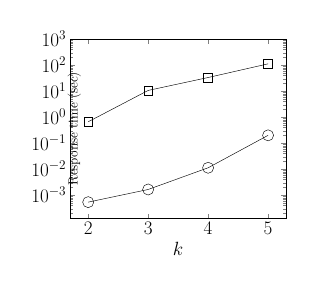
\begin{tikzpicture}[scale=0.4]
        	\tikzstyle{every node}=[font=\LARGE]
            	\begin{axis}[
            		ymode=log,
					xtick={1,2,3,4,5},
           			max space between ticks=30pt,
					try min ticks = 5,
					xlabel={$k$},
    				ylabel={Response time (sec)},
    				ymax=1000, ymin=0,
    				y label style={
    					at={(axis description cs:-0.03,0.5)},
    					anchor=north,
    					font=\large
    				},
    				legend style={
           				at={(1.1,1.25)},
           				anchor=north,
           				legend columns=-1           			
           			},
					mark size=4pt
				]
				\addplot[color=black,mark=square]   coordinates { % KSP-DML
					(2,0.661175509)		 
					(3,10.63344) 		 
					(4,33.35989)		 
					(5,111.91120)		 
				};
				\addplot[color=black,mark=o,mark size=5pt]  coordinates { % SVP-DML
					(2,0.000537981)		 
					(3,0.00165) 		 
					(4,0.011274305)		 
					(5,0.19930)		 
				};
				%\legend{\kdspalgo,\kdspsvp}				
				\end{axis}
			\end{tikzpicture}
			\caption{Adlershof}
		\end{subfigure}
		%
		\begin{subfigure}[t]{0.49\textwidth}
		%
        \begin{subfigure}[t]{0.49\textwidth }
        	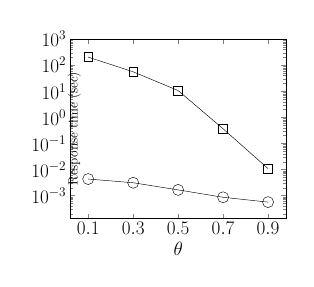
\begin{tikzpicture}[scale=0.4]
        		\tikzstyle{every node}=[font=\LARGE]
        		\begin{axis}[
        			ymode=log,
					xtick={0.1,0.3,0.5,0.7,0.9},
           			max space between ticks=30pt,
					try min ticks = 5,
					xlabel={$\theta$},
    				ylabel={Response time (sec)},
    				ymax=1000, ymin=0,
    				y label style={
    					at={(axis description cs:-0.03,0.5)},
    					anchor=north,
    					font=\large
    				},
					mark size=4pt
				]
				\addplot[color=black,mark=square] coordinates { % KSP-DML
					(0.1,203.74567) 	 
					(0.3,55.76997) 	 
					(0.5,10.63344) 	 
					(0.7,0.36435) 	 
					(0.9,0.01080) 	 
				};
				\addplot[color=black,mark=o,mark size=5pt] coordinates { % SVP-DML
					(0.1,0.004305958) 	 
					(0.3,0.003103674) 	 
					(0.5,0.00165) 	 
					(0.7,0.00086) 	 
					(0.9,0.00056) 	 
				};
				\end{axis}
			\end{tikzpicture}
			\caption{Adlershof}
    	\end{subfigure}
    	%
      	\caption{(a) Response time}
    \end{subfigure}
%%%%%
	\begin{subfigure}[t]{0.49\textwidth}
		%
		\begin{subfigure}[t]{0.49\textwidth}
        	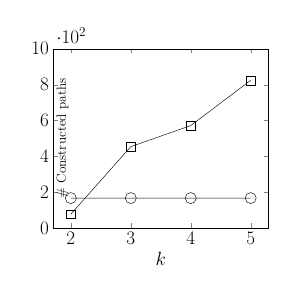
\begin{tikzpicture}[scale=0.4]
        		\tikzstyle{every node}=[font=\LARGE]
            	\begin{axis}[
					xtick={1,2,3,4,5},
           			max space between ticks=30pt,
					try min ticks = 5,
					xlabel={$k$},
    				ylabel={$\#$ Constructed paths},
    				ymax=1000, ymin=0,
    				ytick={0,200,400,600,800,1000},
    				y label style={
    					at={(axis description cs:0,0.5)},
    					anchor=north,
    					font=\large
    				},
    				legend style={
           				at={(1.1,1.25)},
           				anchor=north,
           				legend columns=-1           			
           			},
           			scaled y ticks={base 10:-2},
					mark size=4pt
				]
				\addplot[color=black,mark=square]   coordinates { % KSP-DML
					(2,77.307)		 
					(3,454.16) 		 
					(4,571.63)		 
					(5,824.17)
				};
				\addplot[color=black,mark=o,mark size=5pt]  coordinates { % SVP-DML
					(2,167.315)			 
					(3,167.38) 			 
					(4,167.315)			 
					(5,167.32)			 
				};
				%\legend{\kdspalgo,\kdspsvp,\bsl}						
				\end{axis}
			\end{tikzpicture}
			\caption{Adlershof}
		\end{subfigure}	
		%
        \begin{subfigure}[t]{0.49\textwidth }
        	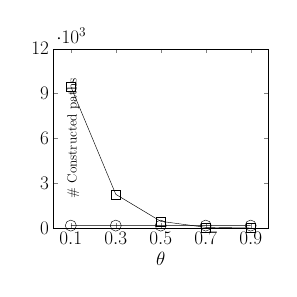
\begin{tikzpicture}[scale=0.4]
        		\tikzstyle{every node}=[font=\LARGE]
        		\begin{axis}[
					xtick={0.1,0.3,0.5,0.7,0.9},
           			max space between ticks=30pt,
					try min ticks = 5,
					xlabel={$\theta$},
    				ylabel={$\#$ Constructed paths},
    				ymax=12000, ymin=0,
    				ytick={0,3000,6000,9000,12000},
    				y label style={
    					at={(axis description cs:0.05,0.5)},
    					anchor=north,
    					font=\large
    				},
    				scaled y ticks={base 10:-3},
					mark size=4pt
				]
				\addplot[color=black,mark=square] coordinates { % KSP-DML
					(0.1,9468.47) 		 
					(0.3,2260.76) 	 
					(0.5,454.16) 	 
					(0.7,51.30) 	 
					(0.9,6.42) 		 
				};
				\addplot[color=black,mark=o,mark size=5pt] coordinates { % SVP-DML
					(0.1,167.315) 		 
					(0.3,167.315) 		 
					(0.5,167.38) 		 
					(0.7,167.32) 		 
					(0.9,167.32) 		 
				};
				\end{axis}
			\end{tikzpicture}
			\caption{Adlershof}
    	\end{subfigure}
    	%
      	\caption{(b) Constructed paths}
    \end{subfigure}
%%%%%
	\caption{Response time of algorithms processing \kdsp queries on Adlershof and Kreuzberg varying requested paths $k$ and similarity threshold $\theta$.}
	\label{fig:kdsp-exp}
\end{figure}

\begin{figure}[htb]
	\centering
	\captionsetup[subfigure]{labelformat=empty}
%%%%%
	\begin{subfigure}[t]{0.49\textwidth}
		%
        \begin{subfigure}[t]{0.49\textwidth}
        	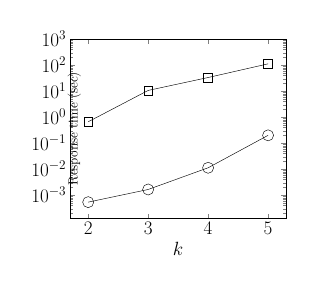
\begin{tikzpicture}[scale=0.4]
        	\tikzstyle{every node}=[font=\LARGE]
            	\begin{axis}[
            		ymode=log,
					xtick={1,2,3,4,5},
           			max space between ticks=30pt,
					try min ticks = 5,
					xlabel={$k$},
    				ylabel={Response time (sec)},
    				ymax=1000, ymin=0,
    				y label style={
    					at={(axis description cs:-0.03,0.5)},
    					anchor=north,
    					font=\large
    				},
    				legend style={
           				at={(1.1,1.25)},
           				anchor=north,
           				legend columns=-1           			
           			},
					mark size=4pt
				]
				\addplot[color=black,mark=square]   coordinates { % KSP-DML
					(2,0.661175509)		 
					(3,10.63344) 		 
					(4,33.35989)		 
					(5,111.91120)		 
				};
				\addplot[color=black,mark=o,mark size=5pt]  coordinates { % SVP-DML
					(2,0.000537981)		 
					(3,0.00165) 		 
					(4,0.011274305)		 
					(5,0.19930)		 
				};
				%\legend{\kdspalgo,\kdspsvp}				
				\end{axis}
			\end{tikzpicture}
			\caption{{\fontsize{0.25cm}{0cm}\selectfont Varying $k$ ($\theta{=}50\%$)}}
		\end{subfigure}
		%
        \begin{subfigure}[t]{0.49\textwidth }
        	\begin{tikzpicture}[scale=0.4]
        		\tikzstyle{every node}=[font=\LARGE]
        		\begin{axis}[
        			ymode=log,
					xtick={0.1,0.3,0.5,0.7,0.9},
           			max space between ticks=30pt,
					try min ticks = 5,
					xlabel={$\theta$},
    				ylabel={Response time (sec)},
    				ymax=1000, ymin=0,
    				y label style={
    					at={(axis description cs:-0.03,0.5)},
    					anchor=north,
    					font=\large
    				},
					mark size=4pt,
					legend style={
           				at={(1.1,1.25)},
           				anchor=north,
           				legend columns=-1           			
           			},
				]
				\addplot[color=black,mark=square] coordinates { % KSP-DML
					(0.1,203.74567) 	 
					(0.3,55.76997) 	 
					(0.5,10.63344) 	 
					(0.7,0.36435) 	 
					(0.9,0.01080) 	 
				};
				\addplot[color=black,mark=o,mark size=5pt] coordinates { % SVP-DML
					(0.1,0.004305958) 	 
					(0.3,0.003103674) 	 
					(0.5,0.00165) 	 
					(0.7,0.00086) 	 
					(0.9,0.00056) 	 
				};
				\legend{\kdspalgo,\kdspsvp}		
				\end{axis}
			\end{tikzpicture}
			\caption{{\fontsize{0.25cm}{0cm}\selectfont Varying $\theta$ ($k{=}3$)}}
    	\end{subfigure}
    	%
      	\caption{(a) Response time}
    \end{subfigure}
%%%%%
	\begin{subfigure}[t]{0.49\textwidth}
		%
		\begin{subfigure}[t]{0.49\textwidth}
        	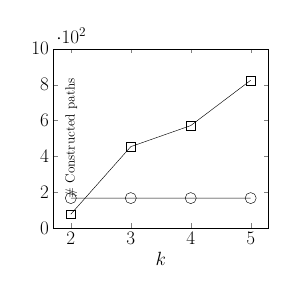
\begin{tikzpicture}[scale=0.4]
        		\tikzstyle{every node}=[font=\LARGE]
            	\begin{axis}[
					xtick={1,2,3,4,5},
           			max space between ticks=30pt,
					try min ticks = 5,
					xlabel={$k$},
    				ylabel={$\#$ Constructed paths},
    				ymax=1000, ymin=0,
    				ytick={0,200,400,600,800,1000},
    				y label style={
    					at={(axis description cs:0.04,0.5)},
    					anchor=north,
    					font=\large
    				},
    				legend style={
           				at={(1.1,1.25)},
           				anchor=north,
           				legend columns=-1           			
           			},
           			scaled y ticks={base 10:-2},
					mark size=4pt
				]
				\addplot[color=black,mark=square]   coordinates { % KSP-DML
					(2,77.307)		 
					(3,454.16) 		 
					(4,571.63)		 
					(5,824.17)
				};
				\addplot[color=black,mark=o,mark size=5pt]  coordinates { % SVP-DML
					(2,167.315)			 
					(3,167.38) 			 
					(4,167.315)			 
					(5,167.32)			 
				};				
				\end{axis}
			\end{tikzpicture}
			\caption{{\fontsize{0.25cm}{0cm}\selectfont Varying $k$ ($\theta{=}50\%$)}}
		\end{subfigure}	
		%
        \begin{subfigure}[t]{0.49\textwidth }
        	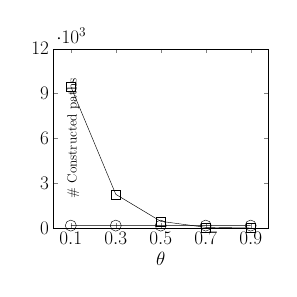
\begin{tikzpicture}[scale=0.4]
        		\tikzstyle{every node}=[font=\LARGE]
        		\begin{axis}[
					xtick={0.1,0.3,0.5,0.7,0.9},
           			max space between ticks=30pt,
					try min ticks = 5,
					xlabel={$\theta$},
    				ylabel={$\#$ Constructed paths},
    				ymax=12000, ymin=0,
    				ytick={0,3000,6000,9000,12000},
    				y label style={
    					at={(axis description cs:0.05,0.5)},
    					anchor=north,
    					font=\large
    				},
    				scaled y ticks={base 10:-3},
					mark size=4pt
				]
				\addplot[color=black,mark=square] coordinates { % KSP-DML
					(0.1,9468.47) 		 
					(0.3,2260.76) 	 
					(0.5,454.16) 	 
					(0.7,51.30) 	 
					(0.9,6.42) 		 
				};
				\addplot[color=black,mark=o,mark size=5pt] coordinates { % SVP-DML
					(0.1,167.315) 		 
					(0.3,167.315) 		 
					(0.5,167.38) 		 
					(0.7,167.32) 		 
					(0.9,167.32) 		 
				};
				\end{axis}
			\end{tikzpicture}
			\caption{{\fontsize{0.25cm}{0cm}\selectfont Varying $\theta$ ($k{=}3$)}}
    	\end{subfigure}
    	%
      	\caption{(b) Constructed paths}
    \end{subfigure}
%%%%%
	\caption{Response time and constructed paths of algorithms \kdspalgo and \kdspsvp on Adlershof varying requested paths $k$ and similarity threshold $\theta$.}
	\label{fig:kdsp-exp}
\end{figure}
